% !TEX program = xelatex
% Compile with XeLaTeX (or LuaLaTeX): pdfLaTeX's T1 fonts have no Vietnamese
% letters such as "ệ" (Việt_Nam, Hà_Nội).
\documentclass[aspectratio=169]{beamer}
\usetheme{Madrid}
\usecolortheme{default}

% Packages
\usepackage{fontspec}
\usepackage{graphicx}
% Figures from docs/figures/, whether compiled from docs/ or the repository root.
\graphicspath{{figures/}{docs/figures/}}
\usepackage{booktabs}
\usepackage{hyperref}

% Title information (the short forms appear in the footline of every slide)
\title[VN-DBpedia Capstone]{Build a DBpedia Version for the Vietnamese Language}
\author[Group 18]{Group 18}
\institute[IT6390E]{Hanoi University of Science and Technology}
\date{\today}

% Title slide colours
\definecolor{titlebg}{HTML}{F8F9F9}
\definecolor{titleink}{HTML}{22343C}
\definecolor{titlemuted}{HTML}{3D4F57}
\newcommand{\monthyear}{\ifcase\month\or January\or February\or March\or April\or May\or
  June\or July\or August\or September\or October\or November\or December\fi\ \number\year}

\begin{document}

% ---------------------------------------------------------
% Title slide: own layout, without the Madrid header and footline
{
\setbeamercolor{background canvas}{bg=titlebg}
\setbeamertemplate{navigation symbols}{}
\begin{frame}[plain, t]
    \color{titleink}
    \vspace*{0.45cm}
    {\fontsize{16.5}{20}\selectfont\bfseries Build a DBpedia Version for the Vietnamese Language\par}
    \vspace{0.3cm}
    {\large\color{titlemuted} Countries from Vietnamese Wikipedia as 5-Star Linked Open Data\par}
    \vspace{0.4cm}
    {\usebeamercolor[fg]{structure}\rule{\linewidth}{1.2pt}}
    \vspace{0.3cm}

    \begin{columns}[T, onlytextwidth]
        \column{0.55\textwidth}
            \textbf{Group 18 members}\par\vspace{0.12cm}
            {\renewcommand{\arraystretch}{1.12}%
            \begin{tabular}{@{}l@{\hspace{1.5em}}l@{}}
                Cao Thi Thu Ha    & 20252264M \\
                Vuong Hoang Minh  & 20252635M \\
                Truong Gia Bach   & 20252277M \\
                Nguyen Thang Phuc & 20252263M \\
            \end{tabular}}
        \column{0.42\textwidth}
            \textbf{Course}\par\vspace{0.12cm}
            IT6390E --- Semantic Web\par
            \vspace{0.35cm}
            \textbf{Supervisor}\par\vspace{0.12cm}
            Dr. Do Ba Lam
    \end{columns}

    \vfill
    Hanoi University of Science and Technology\quad$\cdot$\quad\monthyear
    \vspace*{0.35cm}
\end{frame}
}

% ---------------------------------------------------------
\begin{frame}{Table of Contents}
    \tableofcontents
\end{frame}

% ---------------------------------------------------------
\section{Introduction}
\begin{frame}{Introduction}
    \textbf{The DBpedia Project}
    \begin{itemize}
        \item A global community effort to extract structured knowledge from Wikipedia.
        \item The core of the Linked Open Data (LOD) cloud.
    \end{itemize}
    \vspace{0.5cm}
    \textbf{Motivation for VN-DBpedia}
    \begin{itemize}
        \item While English DBpedia is vast, localized knowledge often lacks structured, semantic representations.
        \item We need a Vietnamese-language Knowledge Graph to power local semantic search, NLP tasks, and regional Linked Data applications.
    \end{itemize}
\end{frame}

% ---------------------------------------------------------
\section{Project Objectives}
\begin{frame}{Project Objectives (Capstone Requirements)}
    \begin{enumerate}
        \item \textbf{Define an Ontology:} Represent country data and relationships semantically.
        \item \textbf{Collect Data:} Scrape infoboxes from Vietnamese Wikipedia.
        \item \textbf{4-Star Data Standard:} Transform collected JSON data into W3C standard RDF.
        \item \textbf{Link to English DBpedia:} Map local entities to the global LOD cloud (achieving 5-star standard).
        \item \textbf{Query Interface:} Host the semantic graph via a SPARQL endpoint.
    \end{enumerate}
\end{frame}

% ---------------------------------------------------------
\section{System Architecture}
\begin{frame}{System Architecture}
    Our pipeline is divided into two primary phases: Data Engineering and Data Hosting.
    \vspace{0.3cm}
    \begin{columns}
        \column{0.5\textwidth}
        \textbf{1. Python Extraction Pipeline}
        \begin{itemize}
            \item \textbf{Discovery:} Wikidata API querying.
            \item \textbf{Extraction:} MediaWiki API (Wikitext to JSON).
            \item \textbf{Transformation:} \texttt{rdflib} generates RDF/Turtle.
        \end{itemize}
        
        \column{0.5\textwidth}
        \textbf{2. SPARQL Hosting Service}
        \begin{itemize}
            \item \textbf{Engine:} Apache Jena Fuseki.
            \item \textbf{Deployment:} Docker Compose.
            \item \textbf{Interface:} Web UI for standard SPARQL querying.
        \end{itemize}
    \end{columns}
\end{frame}

\begin{frame}{Service Architecture}
    \centering
    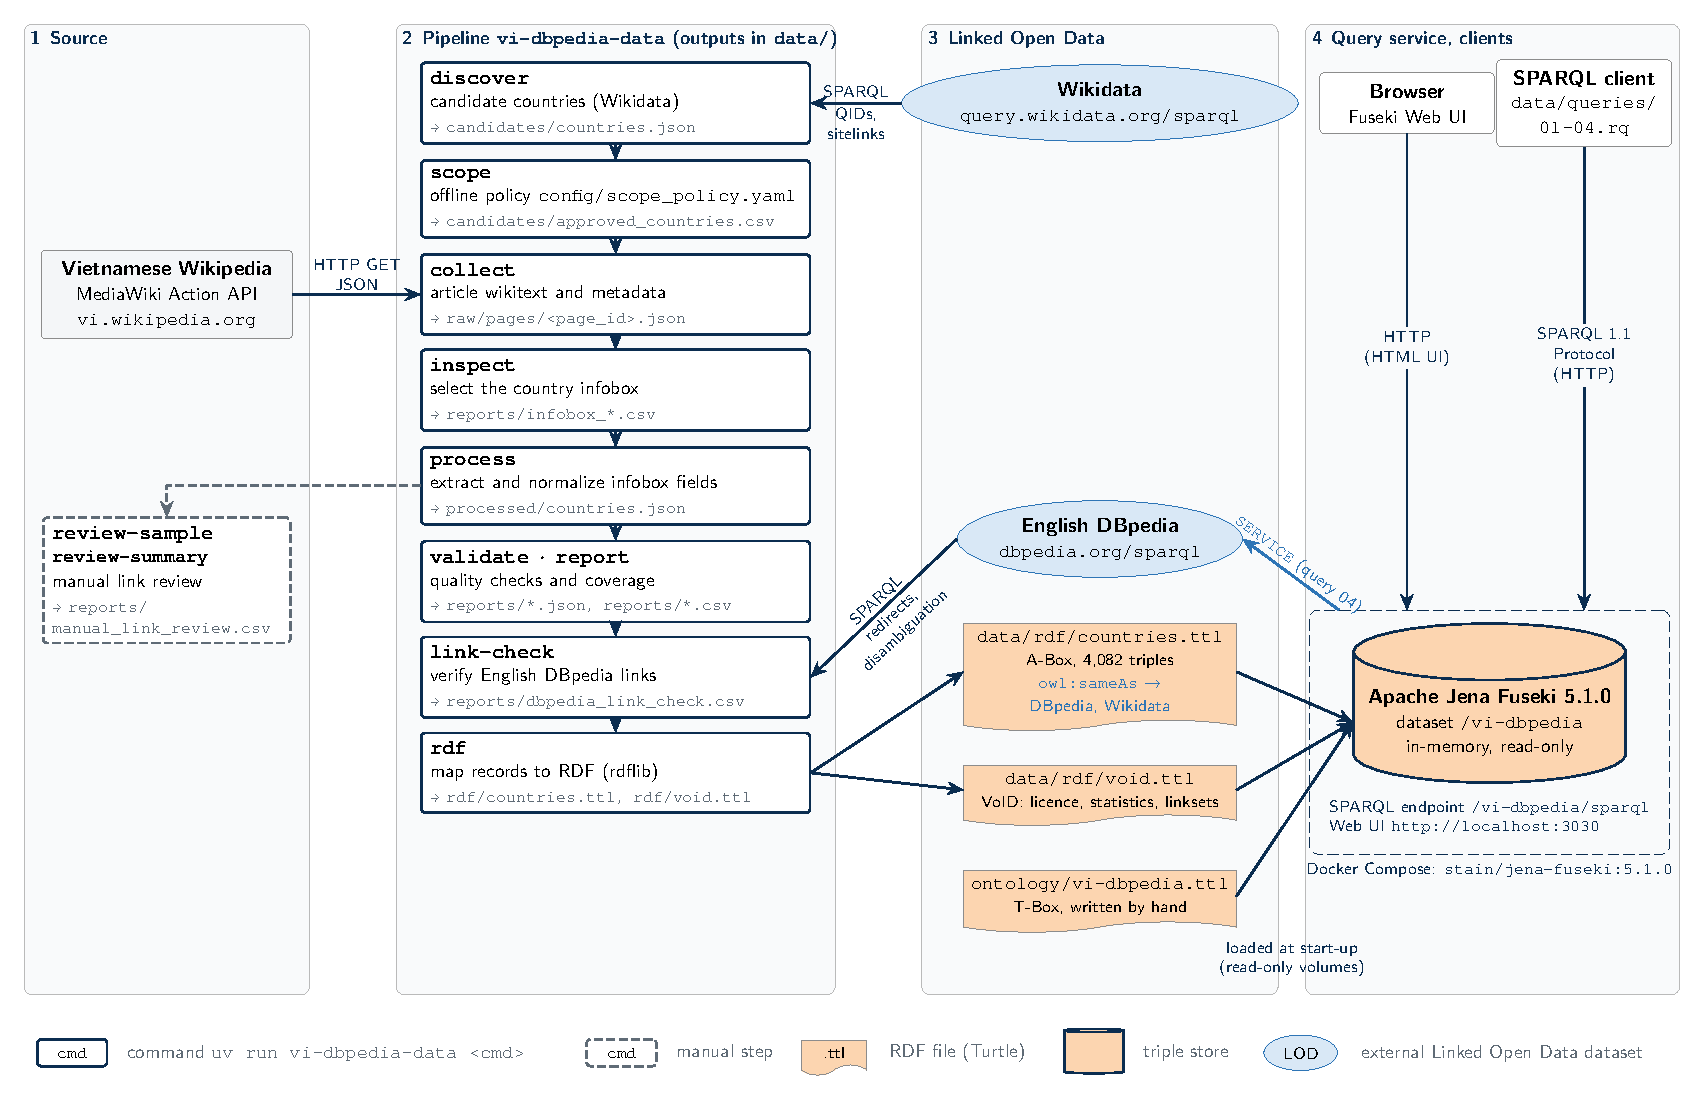
\includegraphics[width=\linewidth, height=0.86\textheight, keepaspectratio]{fig_architecture.pdf}
\end{frame}

% ---------------------------------------------------------
\section{Ontology \& Design}
\begin{frame}{Ontology Design: Reusing DBpedia Standards}
    Instead of inventing proprietary schemas, we reuse the standard DBpedia (\texttt{dbo:}) ontology and add \texttt{vio:} terms only where DBpedia has none (\texttt{ontology/vi-dbpedia.ttl}).
    
    \vspace{0.3cm}
    \begin{table}
        \centering
        \begin{tabular}{@{}lll@{}}
        \toprule
        \textbf{Raw Field} & \textbf{RDF Predicate} & \textbf{Datatype / Object} \\ \midrule
        Entity URI & \texttt{vir:Việt\_Nam} & \texttt{dbo:Country} \\
        Title & \texttt{rdfs:label} & \texttt{Literal (@vi)} \\
        Population & \texttt{dbo:populationTotal} & \texttt{xsd:nonNegativeInteger} \\
        Area ($m^2$) & \texttt{dbo:areaTotal} & \texttt{xsd:double} \\
        Capital & \texttt{dbo:capital} & \texttt{Object URI (vir:Hà\_Nội, dbo:City)} \\
        Calling code & \texttt{vio:callingCode} & \texttt{xsd:string} (new term) \\ \bottomrule
        \end{tabular}
    \end{table}
    
    \textit{Note: All text literals are strictly tagged with \texttt{@vi} for internationalization.}
\end{frame}

\begin{frame}{Ontology (T-Box): \texttt{ontology/vi-dbpedia.ttl}}
    \centering
    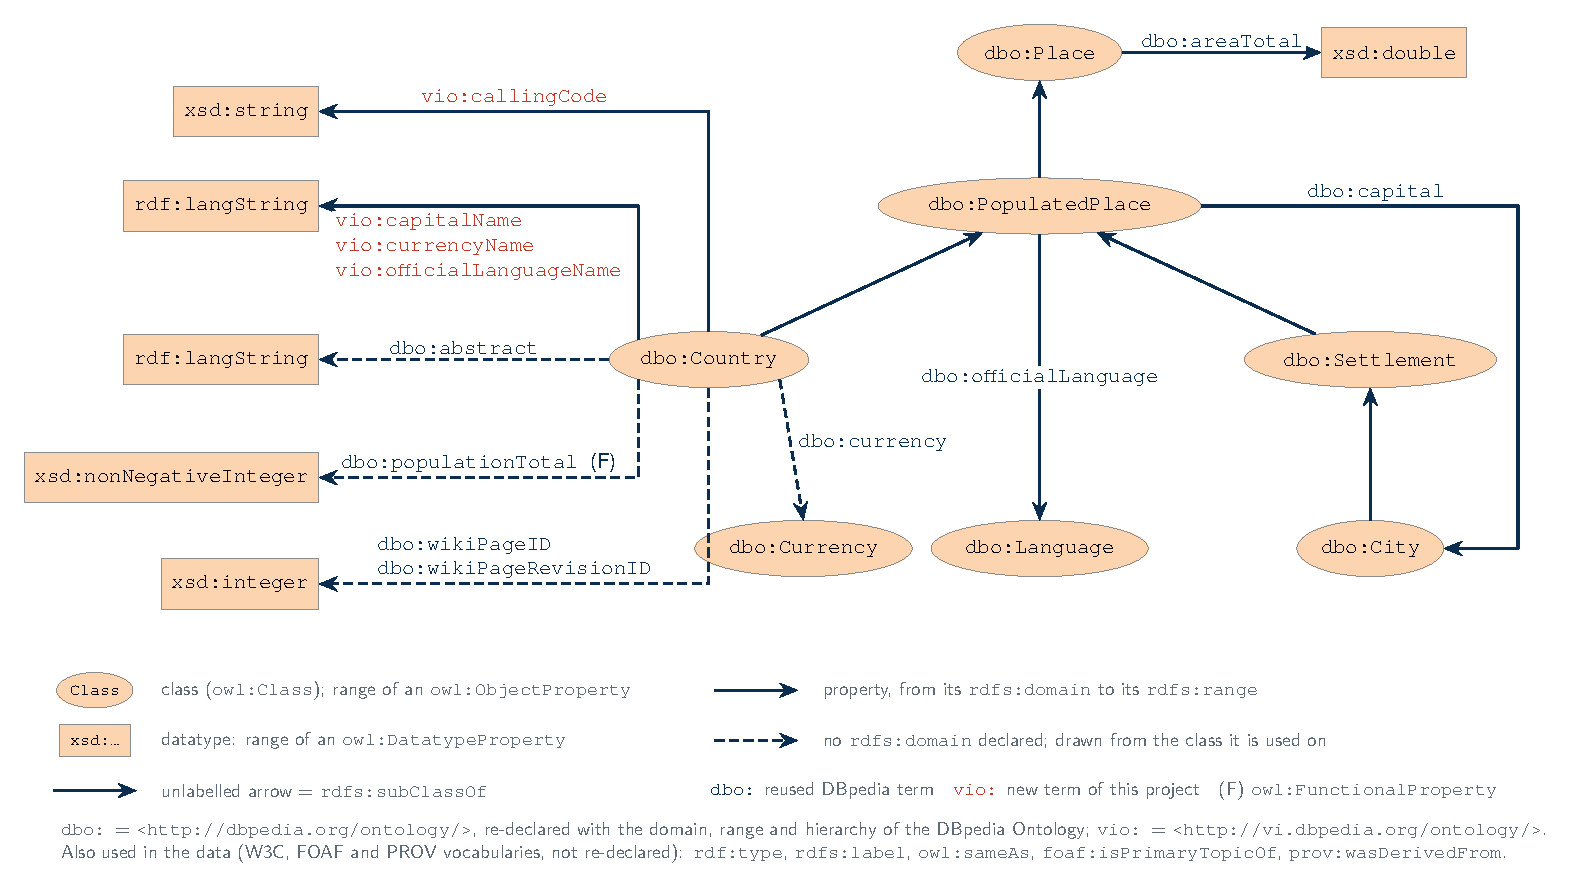
\includegraphics[width=\linewidth, height=0.86\textheight, keepaspectratio]{fig_ontology.pdf}
\end{frame}

\begin{frame}{Data Schema (A-Box): One Country Record}
    \centering
    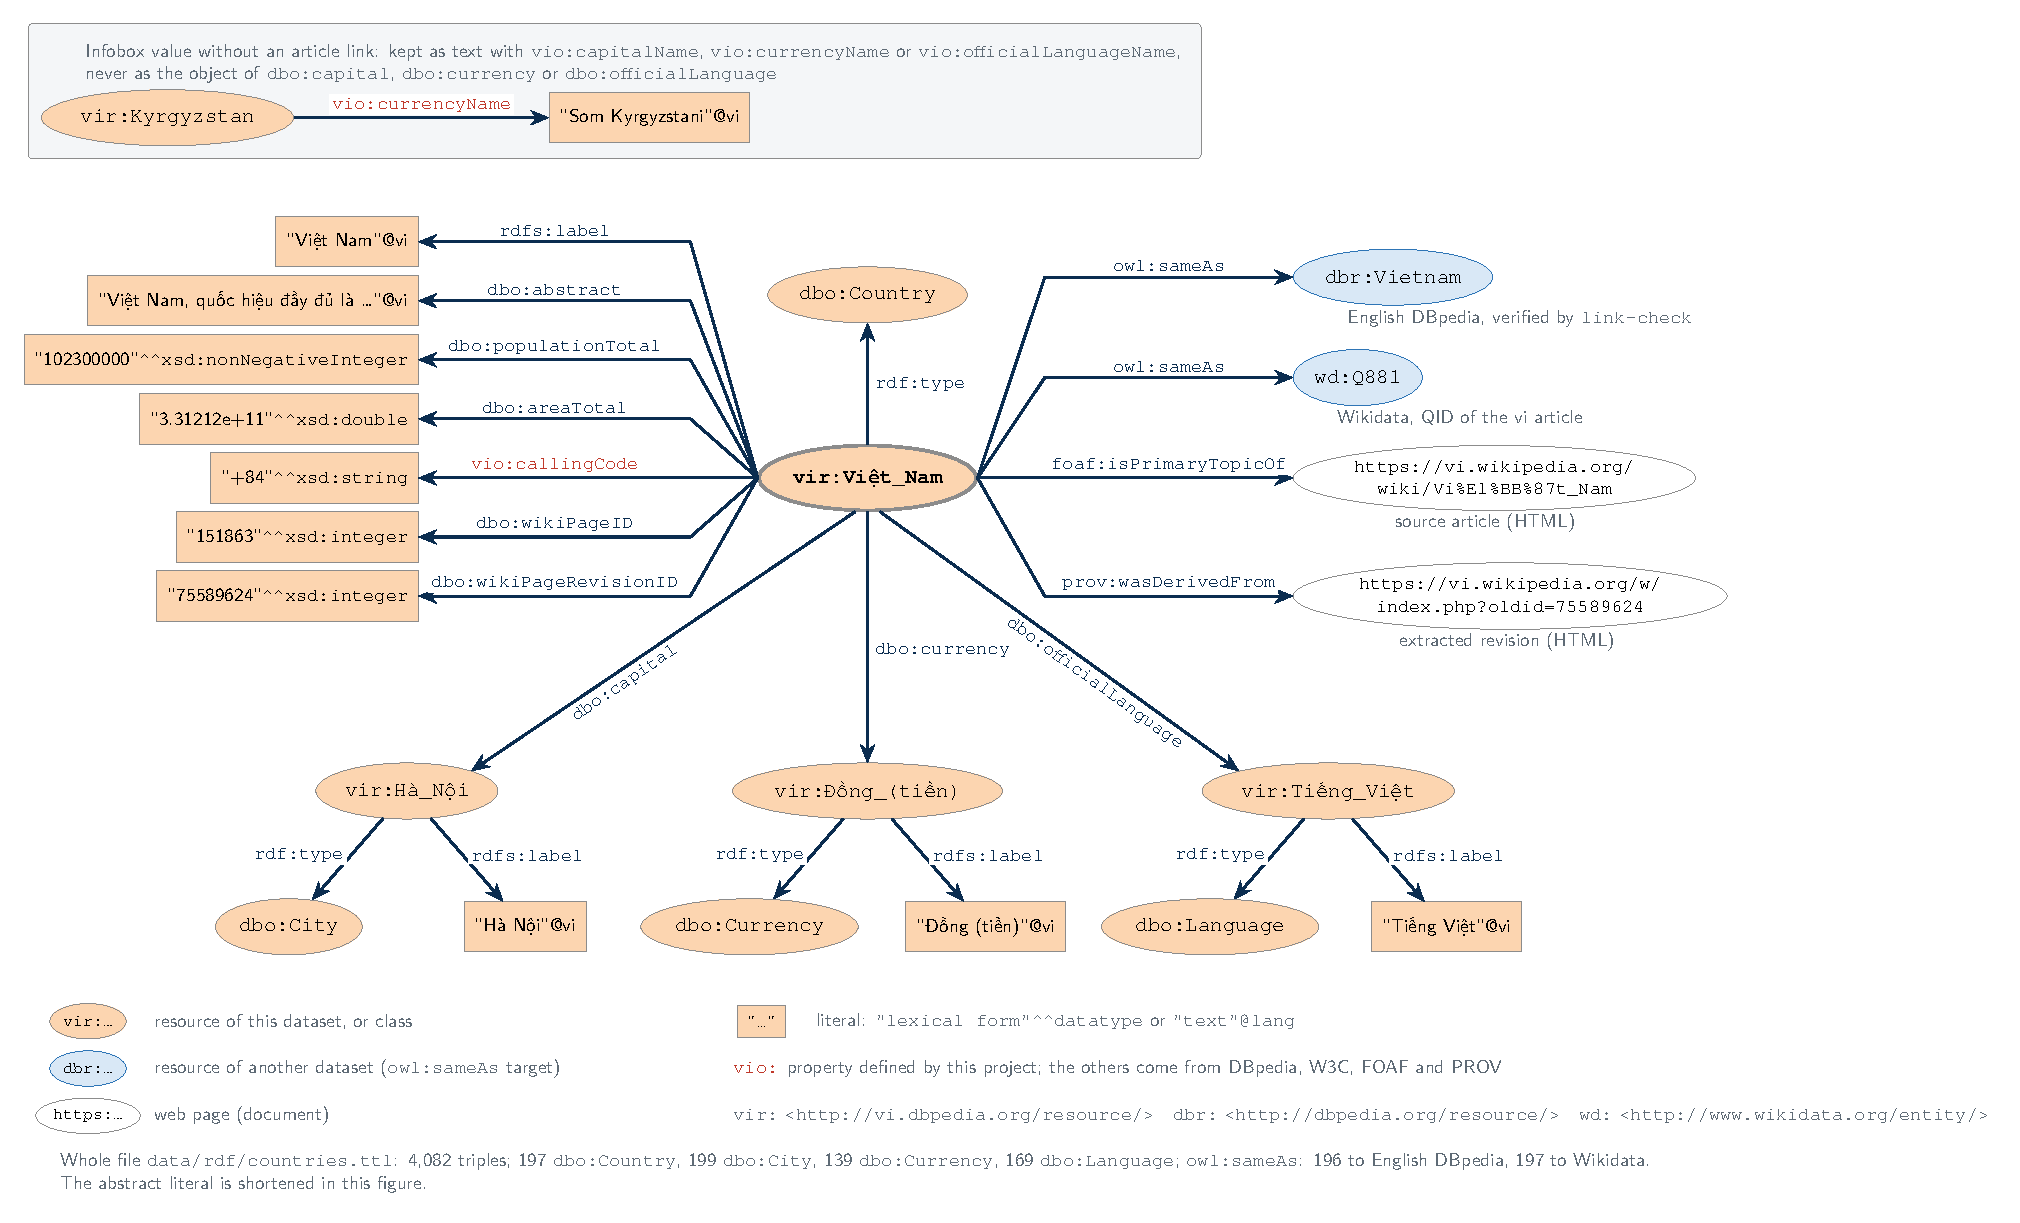
\includegraphics[width=\linewidth, height=0.86\textheight, keepaspectratio]{fig_data_schema.pdf}
\end{frame}

% ---------------------------------------------------------
\section{Achieving 5-Star Linked Data}
\begin{frame}[fragile]{Achieving 4-Star and 5-Star Linked Data}
    \textbf{4-Star Data (RDF Serialization)} \\
    Data is published in non-proprietary Turtle (\texttt{.ttl}) format with strict typing.
    
    \vspace{0.3cm}
    \textbf{5-Star Data (Cross-Lingual Linking)} \\
    English DBpedia links come from Wikipedia interlanguage links, verified against the DBpedia SPARQL endpoint (redirects resolved, disambiguation pages dropped); every country is also linked to Wikidata.

    % semiverbatim, not listings: listings garbles Vietnamese letters such as "ệ".
    \begin{exampleblock}{Turtle (\texttt{data/rdf/countries.ttl})}
    \footnotesize
\begin{semiverbatim}
vir:Việt_Nam a dbo:Country ;
    rdfs:label "Việt Nam"@vi ;
    dbo:populationTotal "102300000"^^xsd:nonNegativeInteger ;
    owl:sameAs dbr:Vietnam , wd:Q881 .
\end{semiverbatim}
    \end{exampleblock}
\end{frame}

% ---------------------------------------------------------
\section{Results \& Query Interface}
\begin{frame}{Results \& Query Interface}
    \textbf{Dataset Metrics:}
    \begin{itemize}
        \item \textbf{197} Sovereign States processed.
        \item \textbf{4,082} RDF triples describing \textbf{704} typed entities.
        \item \textbf{196/197} verified links to English DBpedia, \textbf{197/197} to Wikidata.
    \end{itemize}
    
    \vspace{0.3cm}
    \textbf{SPARQL Web Service:}
    \begin{itemize}
        \item Hosted entirely on a local Dockerized Apache Jena Fuseki server.
        \item Allows users to run advanced relational, filter-based, and mathematical graph queries instantaneously.
    \end{itemize}
\end{frame}

% ---------------------------------------------------------
\section{Conclusion}
\begin{frame}{Conclusion}
    \textbf{Summary}
    \begin{itemize}
        \item Successfully mapped unstructured Vietnamese Wikitext into a formal, 5-Star Semantic Web graph.
        \item Fulfilled all 5 capstone requirements.
    \end{itemize}
    
    \vspace{0.3cm}
    \textbf{Future Work}
    \begin{itemize}
        \item Expand the pipeline domain (e.g., Cities, People, Organizations).
        \item Implement automated daily syncs with Wikipedia updates.
    \end{itemize}
\end{frame}

% ---------------------------------------------------------
\begin{frame}
    \begin{center}
        \Huge \textbf{Thank You} \\
        \vspace{0.5cm}
        \Large Q \& A
    \end{center}
\end{frame}

\end{document}

